\chapter{SYSTEM DESIGN}

\section{Use Case Diagram}

The use case diagram represents the interactions between different actors and the system. It shows how buyers, sellers, and administrators interact with the Vehicle Bidding System.

\begin{figure}[H]
    \centering
    \begin{tikzpicture}[scale=1.0]
        % Draw the system boundary
        \draw (0,0) rectangle (12,10);
        \node at (6, 10.3) {\textbf{Vehicle Bidding System}};
        
        % Draw actors
        \node[ellipse, draw, minimum width=1.5cm, minimum height=1cm] (buyer) at (-1.5, 7) {Buyer};
        \node[ellipse, draw, minimum width=1.5cm, minimum height=1cm] (seller) at (-1.5, 3) {Seller};
        \node[ellipse, draw, minimum width=1.5cm, minimum height=1cm] (admin) at (-1.5, -1) {Admin};
        
        % Draw use cases
        \node[ellipse, draw, minimum width=2.5cm] (register) at (3, 8.5) {Register/Login};
        \node[ellipse, draw, minimum width=2.5cm] (search) at (3, 6.5) {Search Vehicles};
        \node[ellipse, draw, minimum width=2.5cm] (bid) at (3, 4.5) {Place Bid};
        \node[ellipse, draw, minimum width=2.5cm] (message) at (3, 2.5) {Send Message};
        \node[ellipse, draw, minimum width=2.5cm] (list) at (9, 7.5) {List Vehicle};
        \node[ellipse, draw, minimum width=2.5cm] (verify) at (9, 5.5) {Verify Listing};
        \node[ellipse, draw, minimum width=2.5cm] (manage) at (9, 3.5) {Manage Users};
        \node[ellipse, draw, minimum width=2.5cm] (report) at (9, 1.5) {Generate Report};
        
        % Draw associations
        \draw (buyer) -- (register);
        \draw (buyer) -- (search);
        \draw (buyer) -- (bid);
        \draw (buyer) -- (message);
        
        \draw (seller) -- (register);
        \draw (seller) -- (list);
        \draw (seller) -- (message);
        
        \draw (admin) -- (verify);
        \draw (admin) -- (manage);
        \draw (admin) -- (report);
    \end{tikzpicture}
    \caption{Use Case Diagram - Vehicle Bidding System}
    \label{fig:usecase}
\end{figure}

\section{Activity Diagram}

\subsection{Bidding Process Activity Diagram}

The activity diagram below illustrates the flow of the bidding process, from vehicle browsing to bid placement and winner determination.

\begin{figure}[H]
    \centering
    \begin{tikzpicture}[scale=0.9]
        % Start node
        \node[circle, draw, fill=black, minimum size=0.3cm] (start) at (0, 10);
        
        % Activities
        \node[rectangle, draw, minimum width=2.5cm] (browse) at (0, 8.5) {Browse Vehicles};
        \node[rectangle, draw, minimum width=2.5cm] (select) at (0, 7) {Select Vehicle};
        \node[diamond, draw, minimum width=2.5cm] (check) at (0, 5.5) {Can Bid?};
        \node[rectangle, draw, minimum width=2.5cm] (place) at (-2.5, 4) {Place Bid};
        \node[rectangle, draw, minimum width=2.5cm] (error) at (2.5, 4) {Show Error};
        \node[rectangle, draw, minimum width=2.5cm] (notify) at (0, 2.5) {Notify Users};
        \node[rectangle, draw, minimum width=2.5cm] (end) at (0, 1) {Auction Ended};
        
        % End node
        \node[circle, draw, fill=black, minimum size=0.3cm] (finish) at (0, -0.5);
        
        % Arrows
        \draw[->] (start) -- (browse);
        \draw[->] (browse) -- (select);
        \draw[->] (select) -- (check);
        \draw[->] (check) -| node[right] {Yes} (place);
        \draw[->] (check) -| node[left] {No} (error);
        \draw[->] (place) -- (notify);
        \draw[->] (error) -- (notify);
        \draw[->] (notify) -- (end);
        \draw[->] (end) -- (finish);
    \end{tikzpicture}
    \caption{Activity Diagram - Bidding Process}
    \label{fig:activity_bidding}
\end{figure}

\subsection{Vehicle Listing Activity Diagram}

\begin{figure}[H]
    \centering
    \begin{tikzpicture}[scale=0.9]
        % Start node
        \node[circle, draw, fill=black, minimum size=0.3cm] (start) at (0, 10);
        
        % Activities
        \node[rectangle, draw, minimum width=2.5cm] (create) at (0, 8.5) {Create Listing};
        \node[rectangle, draw, minimum width=2.5cm] (upload) at (0, 7) {Upload Images};
        \node[rectangle, draw, minimum width=2.5cm] (submit) at (0, 5.5) {Submit for Review};
        \node[diamond, draw, minimum width=2.5cm] (review) at (0, 4) {Admin Review};
        \node[rectangle, draw, minimum width=2.5cm] (approved) at (-2.5, 2.5) {Listing Active};
        \node[rectangle, draw, minimum width=2.5cm] (rejected) at (2.5, 2.5) {Send Rejection};
        
        % End node
        \node[circle, draw, fill=black, minimum size=0.3cm] (finish) at (0, 1);
        
        % Arrows
        \draw[->] (start) -- (create);
        \draw[->] (create) -- (upload);
        \draw[->] (upload) -- (submit);
        \draw[->] (submit) -- (review);
        \draw[->] (review) -| node[left] {Approved} (approved);
        \draw[->] (review) -| node[right] {Rejected} (rejected);
        \draw[->] (approved) -- (finish);
        \draw[->] (rejected) -- (finish);
    \end{tikzpicture}
    \caption{Activity Diagram - Vehicle Listing Process}
    \label{fig:activity_listing}
\end{figure}

\section{Entity Relationship Diagram}

The ER diagram illustrates the data structure and relationships between different entities in the system.

\begin{figure}[H]
    \centering
    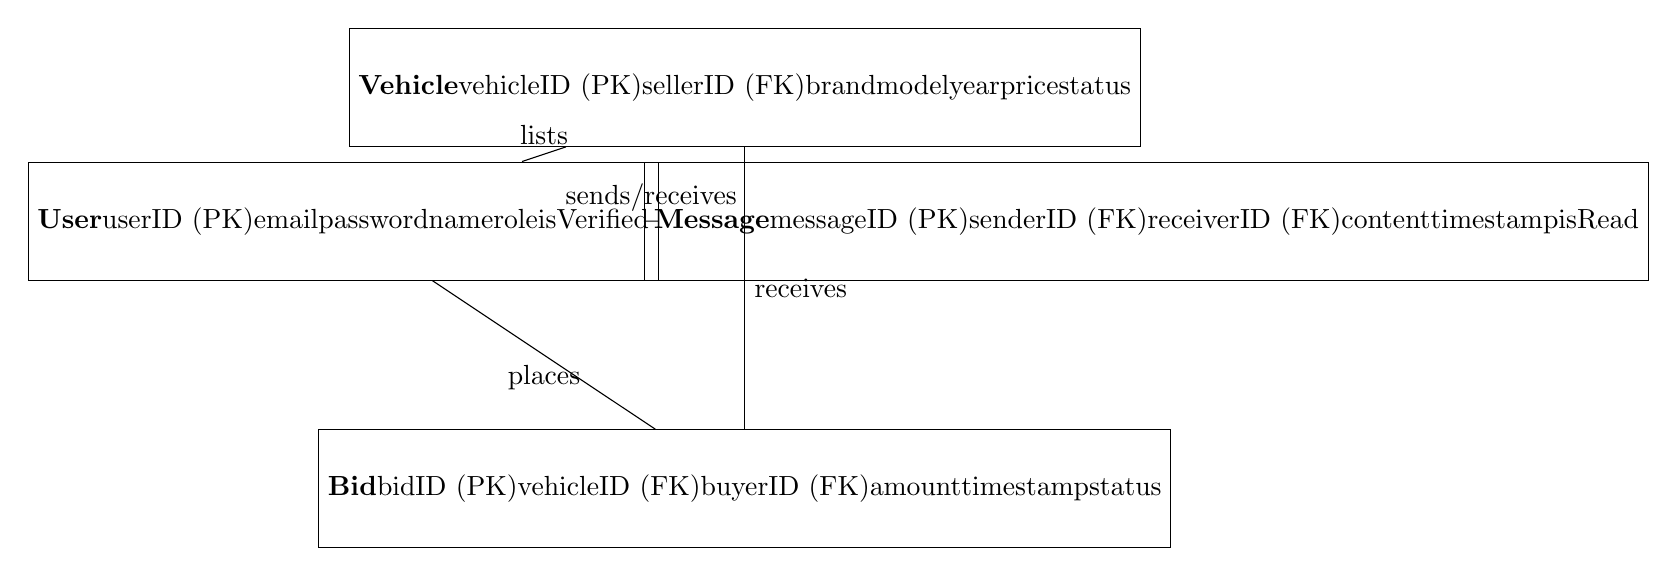
\begin{tikzpicture}[scale=0.85]
        % Define entities
        \node[rectangle, draw, minimum width=2cm, minimum height=1.5cm] (user) at (0, 6) {
            \textbf{User}\\
            userID (PK)\\
            email\\
            password\\
            name\\
            role\\
            isVerified
        };
        
        \node[rectangle, draw, minimum width=2cm, minimum height=1.5cm] (vehicle) at (6, 8) {
            \textbf{Vehicle}\\
            vehicleID (PK)\\
            sellerID (FK)\\
            brand\\
            model\\
            year\\
            price\\
            status
        };
        
        \node[rectangle, draw, minimum width=2cm, minimum height=1.5cm] (bid) at (6, 2) {
            \textbf{Bid}\\
            bidID (PK)\\
            vehicleID (FK)\\
            buyerID (FK)\\
            amount\\
            timestamp\\
            status
        };
        
        \node[rectangle, draw, minimum width=2cm, minimum height=1.5cm] (message) at (12, 6) {
            \textbf{Message}\\
            messageID (PK)\\
            senderID (FK)\\
            receiverID (FK)\\
            content\\
            timestamp\\
            isRead
        };
        
        % Draw relationships
        \draw (user) -- node[above] {lists} (vehicle);
        \draw (vehicle) -- node[right] {receives} (bid);
        \draw (user) -- node[below] {places} (bid);
        \draw (user) -- node[above] {sends/receives} (message);
    \end{tikzpicture}
    \caption{Entity Relationship Diagram}
    \label{fig:erd}
\end{figure}

\section{System Architecture Diagram}

\begin{figure}[H]
    \centering
    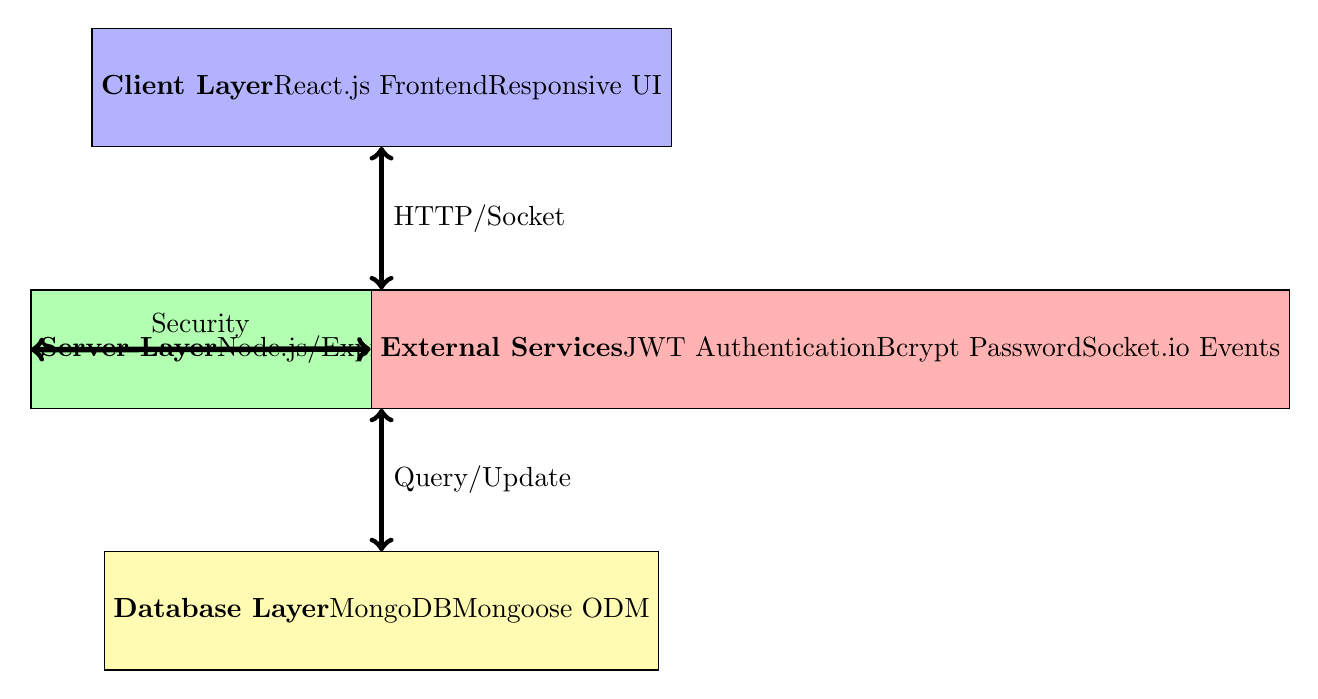
\begin{tikzpicture}[scale=0.95]
        % Client layer
        \node[rectangle, draw, minimum width=3cm, minimum height=1.5cm, fill=blue!30] (client) at (3, 10) {
            \textbf{Client Layer}\\
            React.js Frontend\\
            Responsive UI
        };
        
        % Server layer
        \node[rectangle, draw, minimum width=3cm, minimum height=1.5cm, fill=green!30] (server) at (3, 6.5) {
            \textbf{Server Layer}\\
            Node.js/Express.js\\
            REST API + Socket.io
        };
        
        % Database layer
        \node[rectangle, draw, minimum width=3cm, minimum height=1.5cm, fill=yellow!30] (db) at (3, 3) {
            \textbf{Database Layer}\\
            MongoDB\\
            Mongoose ODM
        };
        
        % External services
        \node[rectangle, draw, minimum width=3cm, minimum height=1.5cm, fill=red!30] (external) at (9, 6.5) {
            \textbf{External Services}\\
            JWT Authentication\\
            Bcrypt Password\\
            Socket.io Events
        };
        
        % Arrows
        \draw[<->, line width=2pt] (client) -- node[right] {HTTP/Socket} (server);
        \draw[<->, line width=2pt] (server) -- node[right] {Query/Update} (db);
        \draw[<->, line width=2pt] (server) -- node[above] {Security} (external);
    \end{tikzpicture}
    \caption{Three-Tier System Architecture}
    \label{fig:architecture}
\end{figure}

\section{Database Schema}

\subsection{User Collection}
\begin{verbatim}
{
  _id: ObjectId,
  email: String (unique),
  password: String (hashed),
  name: String,
  phone: String,
  role: String (buyer/seller/admin),
  isVerified: Boolean,
  profilePicture: String,
  createdAt: Date,
  updatedAt: Date,
  isBlacklisted: Boolean
}
\end{verbatim}

\subsection{Vehicle Collection}
\begin{verbatim}
{
  _id: ObjectId,
  sellerID: ObjectId (ref: User),
  title: String,
  brand: String,
  model: String,
  year: Number,
  price: Number,
  description: String,
  images: [String],
  documents: [String],
  status: String (available/sold/hidden),
  category: String,
  fuelType: String,
  transmission: String,
  mileage: Number,
  auctionEndDate: Date,
  createdAt: Date,
  updatedAt: Date,
  adminVerified: Boolean
}
\end{verbatim}

\subsection{Bid Collection}
\begin{verbatim}
{
  _id: ObjectId,
  vehicleID: ObjectId (ref: Vehicle),
  buyerID: ObjectId (ref: User),
  amount: Number,
  timestamp: Date,
  status: String (active/withdrawn/won/lost),
  isAutomaticBid: Boolean
}
\end{verbatim}

\subsection{Message Collection}
\begin{verbatim}
{
  _id: ObjectId,
  senderID: ObjectId (ref: User),
  receiverID: ObjectId (ref: User),
  vehicleID: ObjectId (ref: Vehicle),
  content: String,
  timestamp: Date,
  isRead: Boolean,
  attachments: [String]
}
\end{verbatim}

\section{API Design}

\subsection{Authentication Endpoints}
\begin{itemize}
    \item \texttt{POST /api/auth/register} - User registration
    \item \texttt{POST /api/auth/login} - User login
    \item \texttt{POST /api/auth/logout} - User logout
    \item \texttt{POST /api/auth/refresh-token} - Refresh JWT token
    \item \texttt{POST /api/auth/forgot-password} - Password reset request
\end{itemize}

\subsection{Vehicle Endpoints}
\begin{itemize}
    \item \texttt{GET /api/vehicles} - Get all vehicles
    \item \texttt{POST /api/vehicles} - Create new vehicle listing
    \item \texttt{GET /api/vehicles/:id} - Get vehicle details
    \item \texttt{PUT /api/vehicles/:id} - Update vehicle listing
    \item \texttt{DELETE /api/vehicles/:id} - Delete vehicle listing
    \item \texttt{GET /api/vehicles/search} - Search vehicles
\end{itemize}

\subsection{Bidding Endpoints}
\begin{itemize}
    \item \texttt{POST /api/bids} - Place a bid
    \item \texttt{GET /api/bids/:vehicleId} - Get all bids for a vehicle
    \item \texttt{GET /api/bids/history/:userId} - Get user's bid history
    \item \texttt{DELETE /api/bids/:bidId} - Withdraw a bid
\end{itemize}

\subsection{Message Endpoints}
\begin{itemize}
    \item \texttt{POST /api/messages} - Send a message
    \item \texttt{GET /api/messages/:userId} - Get user's messages
    \item \texttt{GET /api/messages/conversation/:userId} - Get conversation with user
    \item \texttt{PUT /api/messages/:messageId/read} - Mark message as read
\end{itemize}

\subsection{Admin Endpoints}
\begin{itemize}
    \item \texttt{GET /api/admin/dashboard} - Get dashboard statistics
    \item \texttt{GET /api/admin/listings} - Get pending listings for verification
    \item \texttt{POST /api/admin/listings/:id/verify} - Verify a listing
    \item \texttt{POST /api/admin/users/:id/blacklist} - Blacklist a user
    \item \texttt{GET /api/admin/reports} - Get system reports
\end{itemize}

\section{UI/UX Design}

\subsection{Key Pages}
\begin{itemize}
    \item \textbf{Home Page:} Landing page with featured vehicles and quick search
    \item \textbf{Browse/Search Page:} Vehicle listing with filters and sorting options
    \item \textbf{Vehicle Details Page:} Comprehensive vehicle information with bidding interface
    \item \textbf{Bidding Interface:} Real-time bid placement and history display
    \item \textbf{User Dashboard:} Personal vehicles, bids, and messages
    \item \textbf{Messaging Interface:} Real-time chat with buyers/sellers
    \item \textbf{Admin Dashboard:} System statistics and management tools
    \item \textbf{Seller Dashboard:} Vehicle listing management and analytics
\end{itemize}

\subsection{Design Principles}
\begin{itemize}
    \item Responsive design for desktop, tablet, and mobile devices
    \item Consistent color scheme and typography throughout
    \item Intuitive navigation with clear call-to-action buttons
    \item Real-time feedback for user actions
    \item Accessibility compliance (WCAG 2.1 AA)
    \item Fast loading times and optimized performance
\end{itemize}

\section{Security Design}

\subsection{Authentication}
\begin{itemize}
    \item JWT-based token authentication
    \item Bcrypt password hashing (salt rounds: 10)
    \item Secure session management with token refresh mechanism
    \item Password reset via email verification
\end{itemize}

\subsection{Authorization}
\begin{itemize}
    \item Role-based access control (RBAC)
    \item Middleware to verify user roles and permissions
    \item Resource-level authorization checks
\end{itemize}

\subsection{Data Security}
\begin{itemize}
    \item HTTPS/TLS encryption for all communications
    \item Input validation and sanitization
    \item Protection against SQL injection and XSS attacks
    \item CORS configuration to prevent unauthorized access
    \item Database connection pooling with encryption
\end{itemize}

\subsection{API Security}
\begin{itemize}
    \item Rate limiting to prevent brute force attacks
    \item API key validation for external service calls
    \item Request/response size limits
    \item Security headers (X-Frame-Options, Content-Security-Policy, etc.)
\end{itemize}

